\section{Results}

\subsection{HDAC6 complex formation models predict capsid breakage robustly}

We aimed to integrate the biochemical interaction mechanisms determined by our collaborators from Patrick Matthias' group at FMI with the mechanics of virus uncoating quantitatively, for example, to determine how many cellular motors per exposed capsid are feasible in vivo, and how their actions will translate to virus uncoating (and eventually, infectivity). Because it was not possible to define all interaction mechanisms unambiguously, we formulated three reaction model schemes for HDAC6 complex formation that incorporate distinct mechanistic hypotheses (Figure \ref{figure:ReactionModelSchemes}). We based one model variant termed "Viral Ub" on the previously available uncoating data \cite{banerjee2014influenza}. It assumes competition between capsid-borne and cellular unanchored ubiquitin (Ub) chains for the zinc finger domain of HDAC6. The two model variants incorporating new biochemical protein interaction results assume that cellular ubiquitin chains either assist with binding of both myosin and dynein motors to HDAC6 (variant "Symmetric"), or only with binding of myosin (variant "Asymmetric").

\begin{figure}
\begin{center}
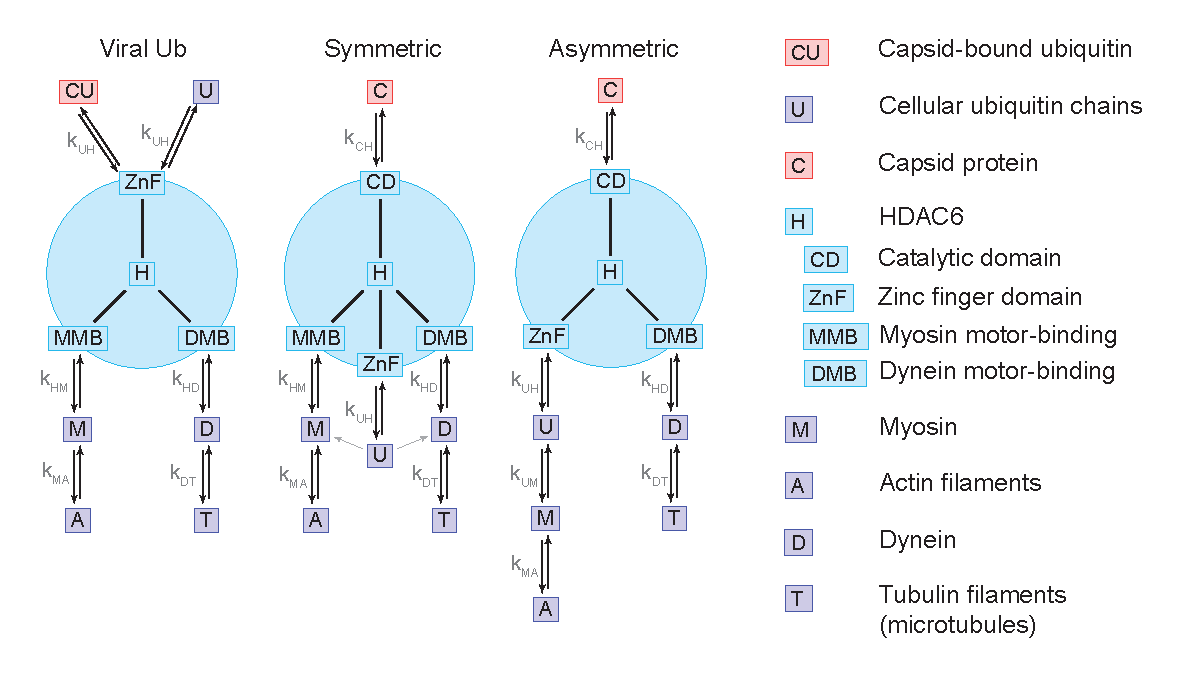
\includegraphics[width=0.95\textwidth, trim={0cm 0cm 0cm 0cm}, clip]{D_chapters/2_ReactionModel/ReactionModels.pdf}
\caption[Interaction schematics for the three reaction model variants]%
{Interaction schematics for the three reaction model variants. Nodes represent proteins or protein domains (linked by solid lines) and arrows denote biochemical reactions with their corresponding on-rates indicated next to the arrows. Node colors distinguish between viral proteins (red), HDAC6 (cyan), and other host proteins (purple).}
\label{figure:ReactionModelSchemes}
\end{center}
\end{figure}

To make the models consistent with prior \textit{in vivo} data, we used published reaction rate parameters for proteins of interest (or averages and similar parameters where data was not available) as well as protein abundances in lung tissues from proteomicsDB \cite{schmidt2018proteomicsdb}. Even when we widely sampled the reaction rate parameters uniformly (with fixed protein concentrations), the "Viral Ub" model failed to generate capsid breakage for any combination of reaction rate parameters. We then optimized unknown and imprecise reaction rate parameters for the other two models to achieve both myosin and dynein recruitment, and thereby maximize breakage, while keeping the reaction rate parameters close to literature values. This yielded reference parameter sets for each model variant. To represent the model uncertainty and to assess its effect on model predictions, we then sampled total protein concentrations normally around the means of previously reported values, and rate parameters log-normally close to their reference values (see Methods for details).

We used the reaction model to compute motor complex abundances for the "Symmetric" and "Asymmetric" model variants at steady state. Both variants can lead to motor complex configurations that are conducive to efficient virus uncoating (see Figure \ref{figure:densitiesRCsupplementary}), but the "Asymmetric" variant leads to higher myosin and dynein binding (Figure \ref{figure:densitiesRC}). Next, we used the mass-spring mechanical model to predict average capsid breakage probabilities from the motor configurations (see Methods). The ‘Asymmetric’ model variant showed a higher density of capsid breakage probabilities close to 100\% for uniform sampling (Figure \ref{figure:densitiesRC} (uniform)), indicating efficient virus uncoating. We obtained qualitatively similar results with a different sampling strategy (Figure \ref{figure:densitiesRC} (normal)). Thus, our models – which incorporate both known constraints and uncertainties – suggest that ubiquitin chains are important for forming motor complexes and thereby for efficient capsid breakage.

\begin{figure}
\begin{center}
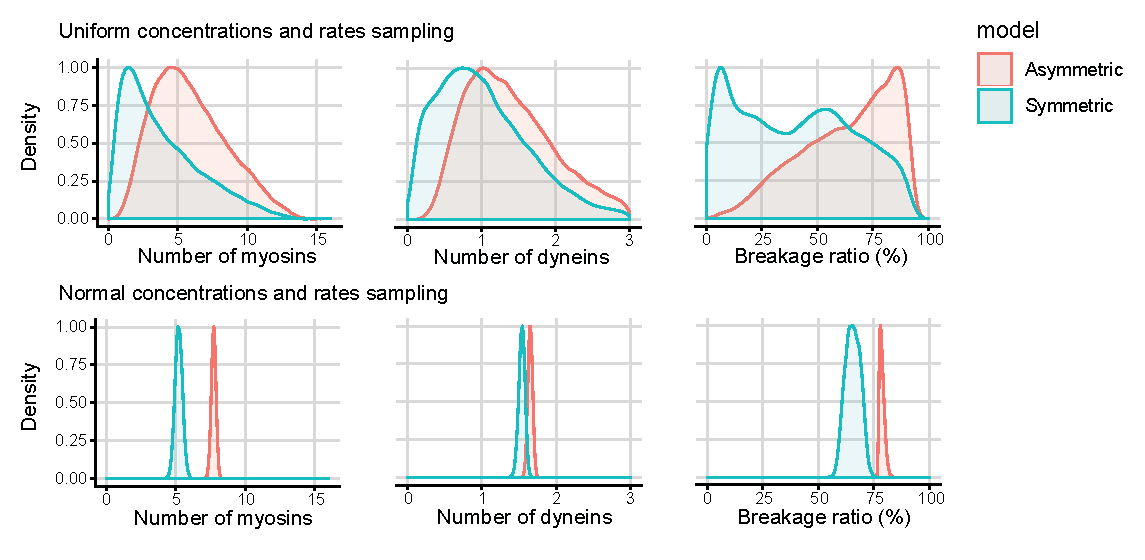
\includegraphics[width=0.95\textwidth, trim={0cm 0cm 0cm 0cm}, clip]{D_chapters/2_ReactionModel/densitiesRC.pdf}
\caption[Molecular motor and capsid breakage density distributions based on joined sampling of rates and concentrations]%
{Density distributions of number of myosin motors (left), number of dynein motors (middle), and capsid breakage probabilities (right) for the ‘Symmetric’ and ‘Asymmetric’ reaction model variants. Initial concentrations and reaction rate constants were sampled uniformly or normally around literature values and rate constant values were adjusted accordingly. The ‘Asymmetric’ model variant allows for relatively high amounts of myosins and dyneins, and total highest breakage probability (see Methods for details). All the densities were normalized by their peak for easier comparison.}
\label{figure:densitiesRC}
\end{center}
\end{figure}

\begin{figure}
\begin{center}
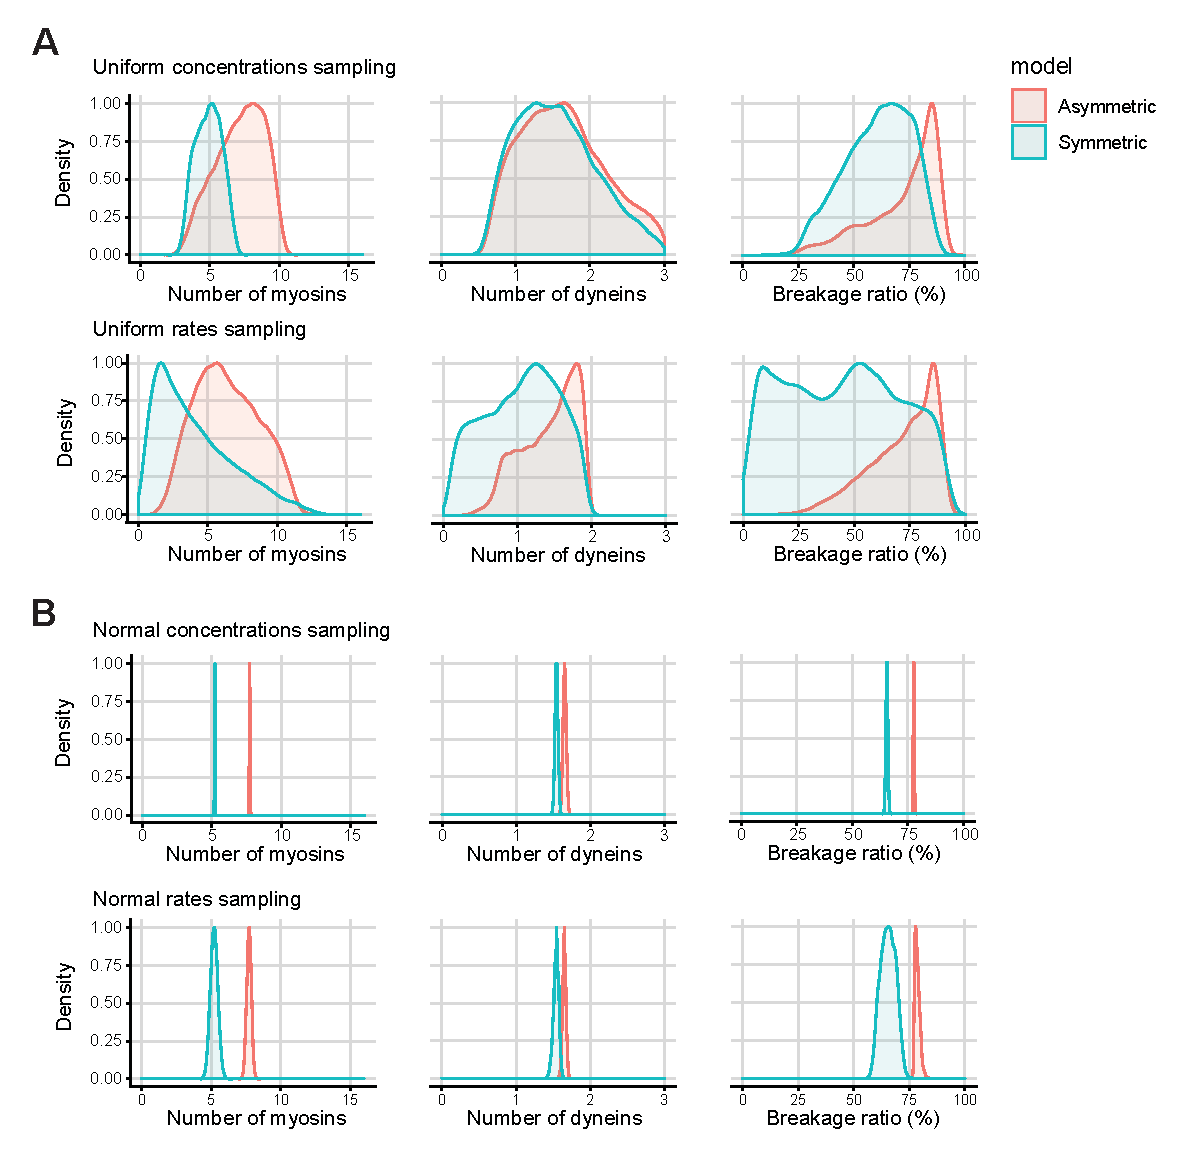
\includegraphics[width=0.95\textwidth, trim={0cm 0cm 0cm 0cm}, clip]{D_chapters/2_ReactionModel/densitiesRCsupplementary.pdf}
\caption[Molecular motor and capsid breakage density distributions based on joined sampling of rates or concentrations]%
{Reaction models' density profiles for the numbers of myosin and dynein motors and for the estimated capsid breakage ratio for (A) uniformly or (B) normally jointly sampled rates or concentrations. All the densities were normalized by their peak for easier comparison.}
\label{figure:densitiesRCsupplementary}
\end{center}
\end{figure}

To identify critical factors for efficient virus uncoating, we varied individual total protein concentrations and rate parameters (Figure 4C, D). Both model variants showed similar sensitivities in the examined ranges. The capsid breakage probability was not sensitive to changes of capsid protein M1 abundance (due to averaging by the number of virions). A decrease in tubulin concentrations led to a weak increase in capsid breakage. In contrast, we observed a peak close to the reference point for dynein, myosin, and HDAC6 concentrations, suggesting an optimal abundance of these proteins for uncoating. For the "Asymmetric" model, changes in ubiquitin elicited a similar peak-like shape, while for the "Symmetric" variant, we observed a plateau. This trend is reversed for the model variants’ actin dependencies. For most of the on-rates, capsid breakage is largely insensitive to changes of reaction rate parameters. However, the "Asymmetric" model is not sensitive to changes in  $k_{CH}$, but sensitive to low values of $k_{UH}$. The reverse holds for the "Symmetric" model. Dissociation constants did not affect capsid breakage at low values, then, sometimes, reached a small peak, and dropped dramatically. One notable difference between the models is that in the "Asymmetric" ("Symmetric") case, $K_{UH}$ ($K_{HM}$) peaks near the reference point, which can be explained by those two reaction rates controlling HDAC6-myosin binding, respectively. Overall, we conclude that our models that combine the biochemistry and mechanics of HDAC6-mediated uncoating can yield robust predictions of capsid breakage in vivo, based on the identified mechanism with asymmetric influence of ubiquitin chains on motor binding.

\subsection{The models predict in vivo responses to host pathway perturbations}

To assess to what extent the model predictions match with independent experimental observations \textit{in vivo}, namely previously published virus uncoating data \cite{banerjee2014influenza}, we first analyzed how uncoating efficiency is affected by perturbations in components of the host cell. We generated predictions with both model variants after introducing model perturbations that correspond to, or are at least similar to, the experimental perturbations (see Methods and Table S3). Specifically, most of the proposed perturbations are relatively straightforward to incorporate, by assuming a reduction of available reactants. For CiliobrevinD, we assume that immobile dyneins do not contribute to capsid breakage (technically it is possible that these fixed motors exert force by holding the capsid protein matrix in place). We represent protein domain mutations – HDAC6 $\Delta$DMC MEF cell line and HDAC6 ZnFm (W1116A) MEF cell line – through increased dissociation constants between HDAC6 and dynein ($K_{HM}$) or ubiquitin ($K_{UH}$), motivated by the model being sensitive to changes in these parameters (Figure \ref{figure:sampledTrajectories}).

\begin{figure}
\begin{center}
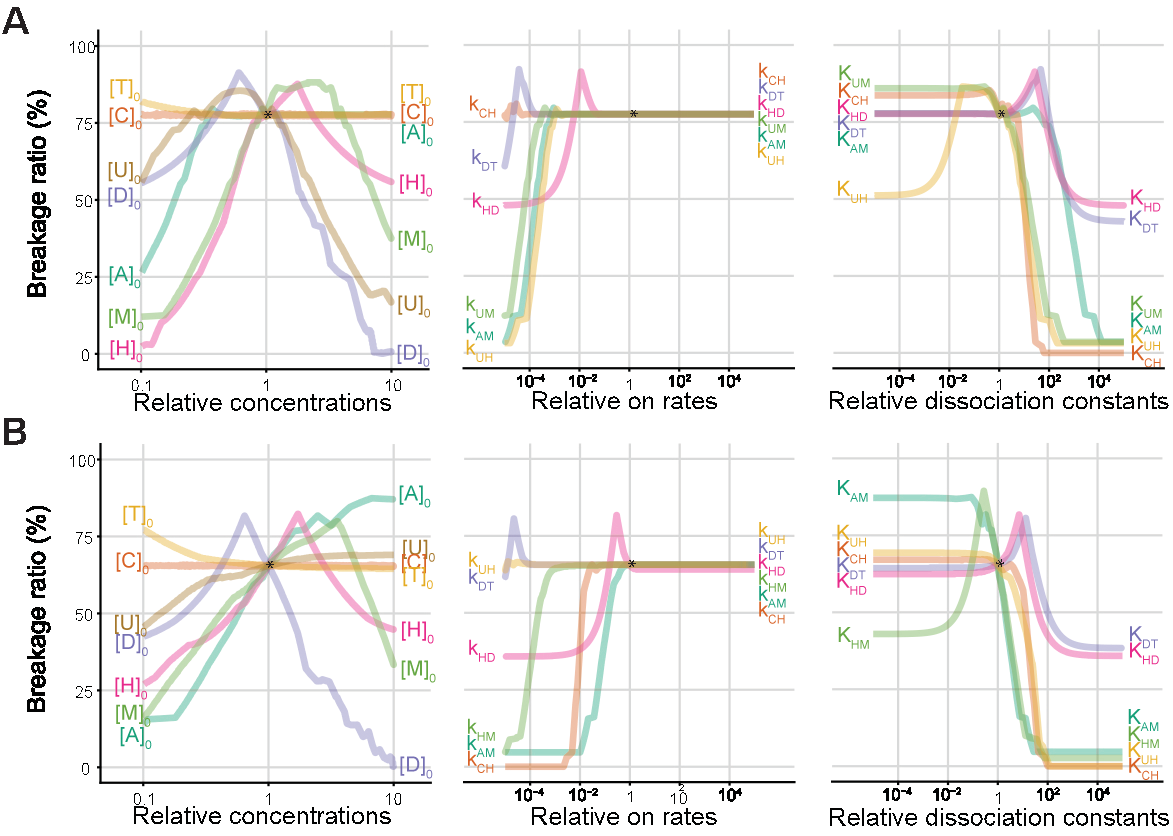
\includegraphics[width=0.95\textwidth, trim={0cm 0cm 0cm 0cm}, clip]{D_chapters/2_ReactionModel/SampledTrajectories.pdf}
\caption[Influence of varying individual initial protein abundances and reaction rate parameters on the capsid breakage probability]%
{Influence of varying individual initial protein abundances and reaction rate parameters on the capsid breakage probability for the "Asymmetric" (A) and ‘Symmetric’ (B) model. All the varied parameters were normalized by the values corresponding to the reference conditions.}
\label{figure:sampledTrajectories}
\end{center}
\end{figure}

First, we focused on perturbations of the host cell’s molecular motors. Experimental data on virus uncoating efficiency were obtained in acid bypass assays that mimic normal infection by lowering the extracellular pH and blocking the natural acidification in endosomes \cite{banerjee2014influenza}. For the examined perturbations, the predicted median uncoating efficiencies agree well with the experimental results (Figure \ref{figure:reactionModelPredictions}A). The "Symmetric" predictions were slightly closer to the experimental results.

\begin{figure}
\begin{center}
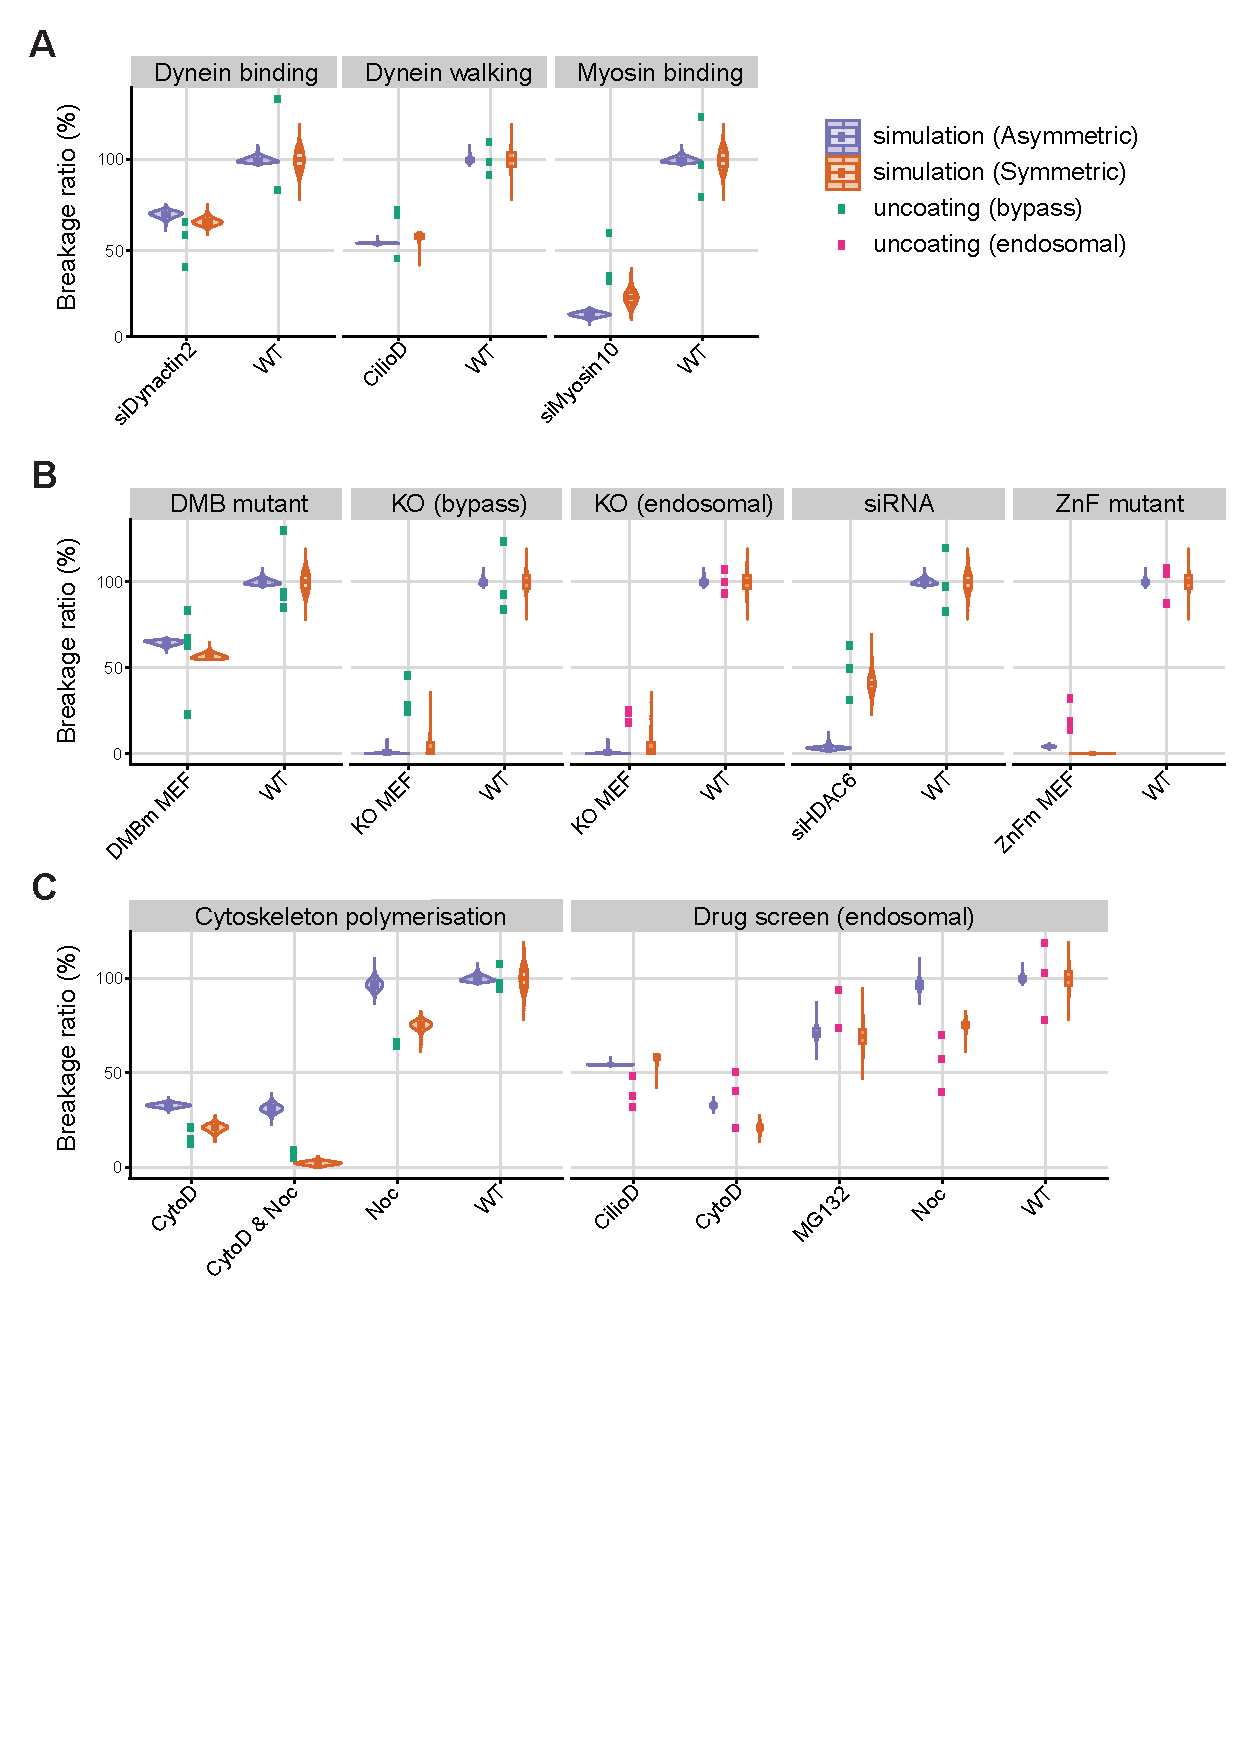
\includegraphics[width=0.8\textwidth, trim={0cm 8.5cm 0cm 0cm}, clip]{D_chapters/2_ReactionModel/FIGURE5_upd2.pdf}
\caption[The model predicts \textit{in vivo} uncoating efficiencies upon perturbations of the host cell]%
{The model predicts \textit{in vivo} uncoating efficiencies upon perturbations of the host cell.\par
Grey labels indicate the type of perturbations, and axis labels the specific experimental conditions.\par
(A) Perturbations of molecular motors.  Abbreviations: WT, wild type; siDynactin2, siRNA for Dynactin2; CilioD, Ciliobrevin D; siMyosin10, siRNA for myosin10. \par
(B) Perturbations of HDAC6. Abbreviations: DMBm, dynein motor binding mutant; KO, knock out; MEF, mouse embryonic fibroblasts; siHDAC6, siRNA for HDAC6; ZnFm, zinc finger mutant.\par
(C) Cytoskeletal perturbations and drug screen for inhibition of endosomal entry. Abbreviations: CytoD, Cytochalasin D; Noc, Nocodazole; CilioD, Ciliobrevin D.\par
All data shown are bypass (emerald) and endosomal (pink) experimental uncoating efficiencies and capsid breakage probabilities predicted by simulation of the "Asymmetric" (purple) and "Symmetric" (orange) reaction model with correspondingly perturbed initial conditions and rate parameters (see Methods \ref{ch:ReactionModelsMethods} for details). Experimental data are from \cite{banerjee2014influenza}. All data are normalized with respect to the untreated WT.
}
\label{figure:reactionModelPredictions}
\end{center}
\end{figure}

For a wide variety of HDAC6 perturbations, including knockdowns and mutations of specific domains, the models’ predictions aligned well with the experimental data (Figure \ref{figure:reactionModelPredictions}B). Notably, predictions were consistent with data from bypass experiments as well as experiments that measured endosomal uncoating in the normal virus infection pathway. Note, however, the difference in predicted viral capsid breakage probability in HDAC6 mutants or siRNA knockdown; the model only represents HDAC6-mediated uncoating, while \textit{in vivo} there are likely additional pathways or mediators capable of assisting in the uncoating \cite{gschweitl2016spopl,huotari2012cullin,miyake2019influenza,su2013pooled,yanguez2018phosphoproteomic}. The "Symmetric" model captured siRNA perturbations better than the "Asymmetric" variant, due to the former being less sensitive to reduction in HDAC6 (Figure \ref{figure:sampledTrajectories}), but the "Asymmetric" prediction for the ZnF mutant was closer to the experimental observation.

We compared model predictions with experimental data from perturbations of the host cell’s cytoskeleton and from an endosomal drug screen \cite{banerjee2014influenza} (Figure \ref{figure:reactionModelPredictions}C). Both variants performed well, with one notable exception: the "Asymmetric" variant did not capture the effect of nocadazole treatment, which is consistent with it being less sensitive to reduction in tubulin concentrations (Figure \ref{figure:sampledTrajectories}). Interestingly, except for nocodazole treatment, the "Asymmetric" variant performed better for endosomal perturbations (Figure \ref{figure:reactionModelPredictions}C, drug screen). Overall, we conclude that the combined model predictions compare well against published experimental data. Even when model limitations make the predictions imprecise, the models at the very least predict the correct direction of the perturbation effect on the viral capsid breakage probability. 

\subsection{Modelling HDAC6 inhibition dependency on M1}

Our collaborators from Mirco Schmolke's group at University of Geneva compared early replication efficacy of a panel of influenza A virus strains in wild type (WT) and HDAC6-deficient A549 lung epithelial cells (Figure \ref{figure:infectivityStrainSpecific}A). Strikingly, a clinical H3N2 isolate from 2013 displayed low dependence on HDAC6 for early replication steps as determined by automated fluorescence microscopy for viral nucleoprotein (NP). Specifically, this H3N2 isolate did not rely on a functional ZnF domain of HDAC6 while a clinical H1N1 isolate (pH1N1) from 2010 did. Inactivating HDAC6 deacetylase activity by a mutation in CD2 affected neither of the isolates (Figure \ref{figure:infectivityStrainSpecific}A). Sequence alignment of M1 from HDAC6-dependent (H1N1) and -independent (H3N2) viral strains revealed a single amino acid substitution (A218T in H3N2) (Figure \ref{figure:infectivityStrainSpecific}B) previously associated with matrix shape \cite{elleman2004m1}. Reversion of the 2003 H3N2 virus (A/Wyoming/03/2003) M1 residue 218 to alanine by reverse genetics restored HDAC6 dependence to a similar extent to H1N1 virus (Figure \ref{figure:infectivityStrainSpecific}A) and reduced particle length (not shown).

\begin{figure}
\begin{center}
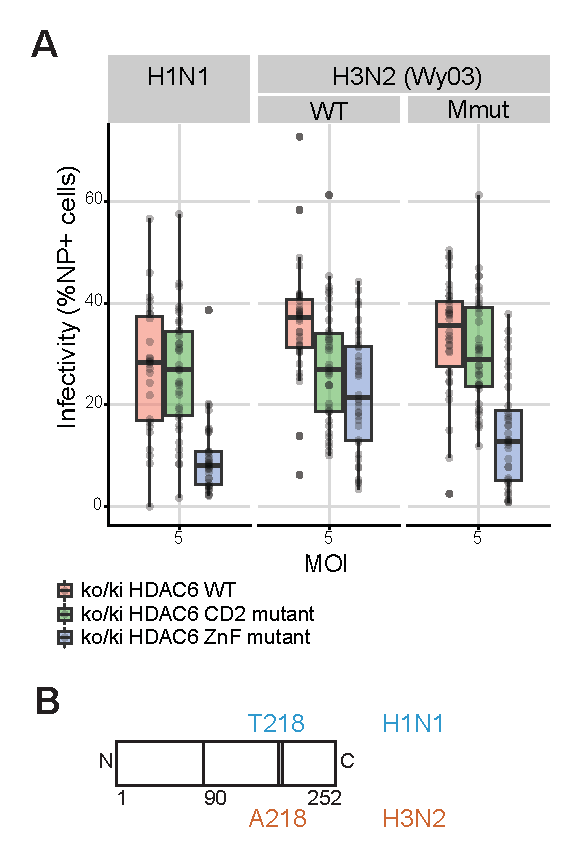
\includegraphics[width=0.7\textwidth, trim={0cm 0cm 0cm 0cm}, clip]{D_chapters/2_ReactionModel/FIGURE6_upd_infectivityStrainSpecific.pdf}
\caption[Influenza H1N1 shows stronger dependence on the HDAC6/aggresome pathway than H3N2]%
{(A) Influenza H1N1 shows stronger dependence on the HDAC6/aggresome pathway than H3N2. 
A549 cells expressing different HDAC6 versions (WT, CD2 mutant or ZnF mutant) were infected with pH1N1 or H3N2 virus at indicated multiplicity of infection (MOI) and cells were stained for viral NP. \par
(B) Schematic of H1N1 vs H3N2 M1, highlighting residue 218.}
\label{figure:infectivityStrainSpecific}
\end{center}
\end{figure}

Our collaborators from Patrick Matthias' group at demonstrated that efficient co-immunoprecipitation of purified C-terminal M1 proteins with HDAC6 depends on alanine at position 218 of M1 (Figure \ref{figure:interactionM1ResidueSpecific}). Specifically, their data suggest that the A218T mutation reduces binding of M1 to HDAC6 by approximately two-fold (Figure \ref{figure:M1ReactionModel}).


\begin{figure}
\begin{center}
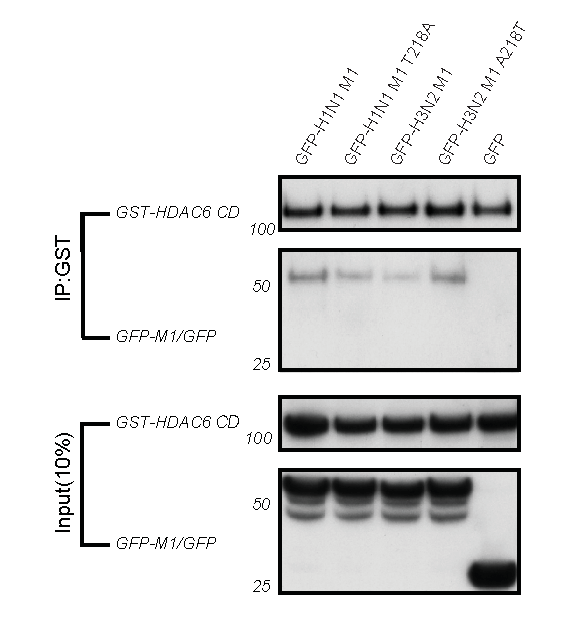
\includegraphics[width=0.8\textwidth, trim={0cm 0cm 0cm 0cm}, clip]{D_chapters/2_ReactionModel/FIGURE6_upd_IP.pdf}
\caption[Preferential interaction of viral H1N1 M1 protein with HDAC6 depends on residue T218.]%
{Preferential interaction of viral H1N1 M1 protein with HDAC6 depends on residue T218.\par
GFP-M1 fusion proteins (H1N1 WT or T218A, H3N2 WT or A218T) were transiently expressed in 293T cells and lysates were incubated with purified GST-HDAC6 (amino acids 82-837, catalytic domains) protein. GST-Trap beads were used to capture HDAC6 and associated proteins. The presence of diverse proteins in the precipitate (IP) or in the input lysate was determined by immunoblotting with anti-GFP (M1) or anti-GST (HDAC6) antibodies.}
\label{figure:interactionM1ResidueSpecific}
\end{center}
\end{figure}

To represent the effect of the amino acid substitution in the reaction models, we assumed that the M1 protein mutation affects the binding between the capsid and HDAC6, specifically the dissociation constant $K_{CH}$. We generated reaction model predictions for the mutant by choosing a multiplication coefficient for both models, setting the desired level of capsid breakage in an individual perturbation experiment (Figure \ref{figure:sampledTrajectories}) to the observed average level of M1 binding (Figure \ref{figure:interactionM1ResidueSpecific}). These model predictions aligned well with the experimental results from \textit{in vitro} M1 pull-down quantification and from in vivo automated fluorescence microscopy for both viral strains and their respective M1 mutants (Figure \ref{figure:M1ReactionModel}). However, the models did not fully capture interactions between different perturbations. For example, the relative infectivity of the pandemic H1N1 (pH1N1) strain in the HDAC6 ko/ki ZnF mutant cells corresponds to a reduction of the binding rate  between the HDAC6 ZnF domain and ubiquitin, and the infectivity of the H3N2 strain in HDAC6 ko/ki WT cells to the increased dissociation rate. Both cases lead to a reduction in capsid breakage. However, our NP fluorescence microscopy data for the H3N2 ko/ki ZnF mutant show a slight increase of viral entry compared to the ko/ki ZnF mutant (Figure \ref{figure:M1ReactionModel}), in contrast to either of the models. To summarize, these results suggest that the models represent key mechanisms of virus uncoating in vivo, despite focusing on only a few biochemical and mechanical interactions between virus and host components.

\begin{figure}
\begin{center}
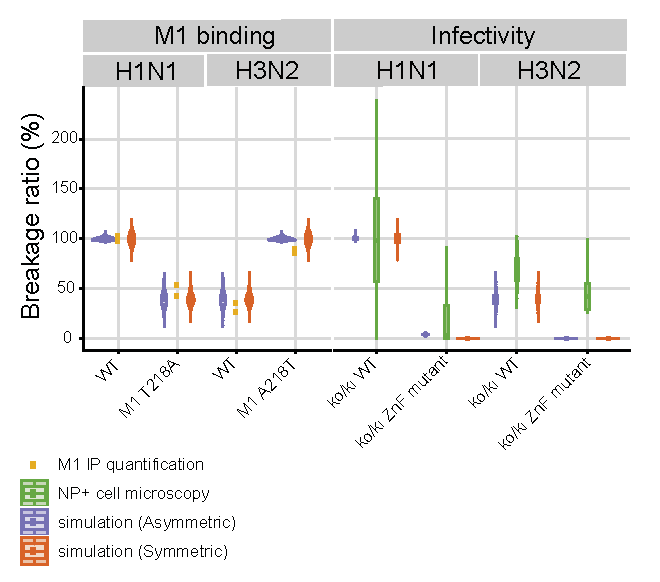
\includegraphics[width=0.8\textwidth, trim={0cm 0cm 0cm 0cm}, clip]{D_chapters/2_ReactionModel/FIGURE6_upd_simulation.pdf}
\caption[The model predictions for uncoating efficiencies based on strength of interaction between influenza M1 and HDAC6]%
{The model predictions for uncoating efficiencies based on strength of interaction between influenza M1 and HDAC6.\par
Experimental M1 IP quantification data from (C, yellow) and NP+ cell microscopy from (B, green) viral activities for perturbations of viral protein M1 variant for H1N1 and H3N2 viruses, compared against capsid breakage probabilities predicted by simulation of the ‘Asymmetric’ (purple) and ‘Symmetric’ (orange) reaction model with correspondingly perturbed initial conditions and rate parameters (see Methods for details). Abbreviations: IP, immunoprecipitation; NP+, nucleoprotein positive; ko/ki, knock out/knock in; WT, wild type; ZnF, zinc finger.
}
\label{figure:M1ReactionModel}
\end{center}
\end{figure}